\section{Cap 6 - Elementos isoparamétricos}

\subsection{Exercícios}

\subsubsection{1) Determinar as funções de interpolação dos elementos}
%
\begin{itemize}
	\item a)
	\begin{figure}[H]
	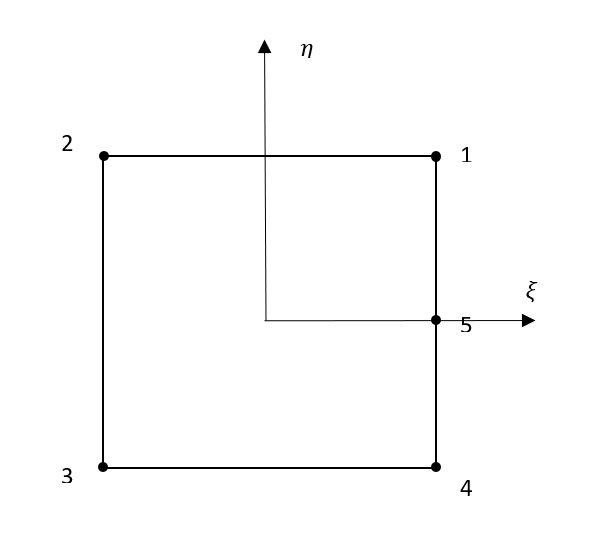
\includegraphics[width=0.6\textwidth,center]{fig/cap6_1_a.PNG}
	\caption{Questão a)} 
	\label{cap6:cap6_1_a}
\end{figure}
%
\end{itemize}
%
As funções de interpolação serão definidas através das funções bilineares. Considerando a Figura \ref{cap6:quad_bilinear_0}, 
%
\begin{figure}[H]
	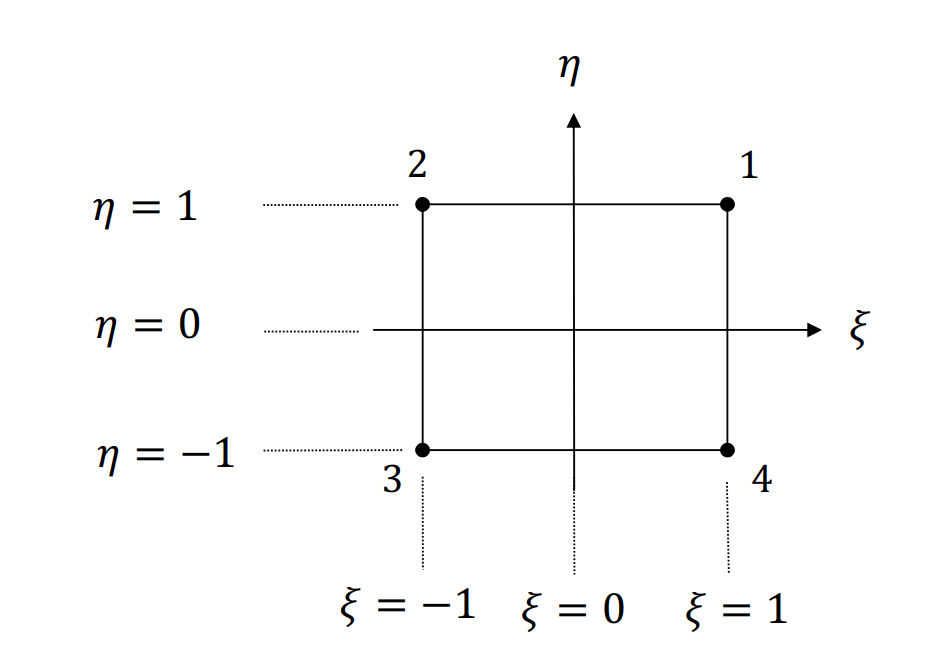
\includegraphics[width=0.6\textwidth,center]{fig/quadrilatero_4_livro.PNG}
	\caption{Parametrização de um elementos quadrilátero bilinear (4 nós)} 
	\label{cap6:quad_bilinear_0}
\end{figure}
%
as funções de interpolações bilineares são,
%
\begin{equation}
	\begin{split}
		&N^b_1(\xi, \eta) = \frac{1}{4}(1 + \xi)(1 + \eta)\\
		&N^b_2(\xi, \eta) = \frac{1}{4}(1 - \xi)(1 + \eta)\\
		&N^b_3(\xi, \eta) = \frac{1}{4}(1 - \xi)(1 - \eta)\\
		&N^b_4(\xi, \eta) = \frac{1}{4}(1 + \xi)(1 - \eta)
	\end{split}
\end{equation}
%
A função de interpolação no ponto 5 é definida como a variação quadrática na direção $\eta$ e linear na direção $\xi$ (Pag. 53). A variação quadrática é obtida pelo polinômio de Lagrange quadrático. Na figura \ref{cap6:Quadratico} temos o elemento que gera a variação quadrática.
%
\begin{figure}[H]
	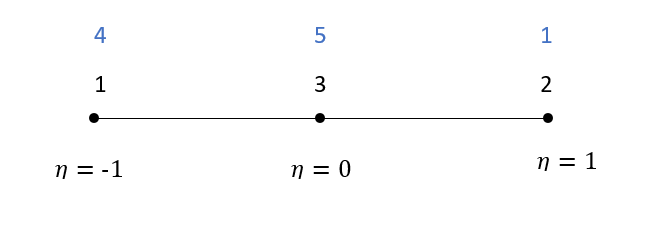
\includegraphics[width=0.6\textwidth,center]{fig/elemento_quad.PNG}
	\caption{Função de interpolação quadrática} 
	\label{cap6:Quadratico}
\end{figure}
%

Na figura \ref{cap6:Quadratico} o ponto 5 equivale ao 3, portanto a variação quadrática é (pag. 49),
%
\begin{equation}
	l^2_3(\eta) = (1-\eta)(1+\eta)
\end{equation}
%
Na variação linear na direção $\xi$ o ponto 5 equivale ao 2 (pag. 49),
%
\begin{equation}
	l^1_2(1+\xi) = \frac{1}{2}(1+\xi)
\end{equation}
%
Assim, o função de interpolação $N_5$ é dada por,
%
\begin{equation}
	N_5(\xi,\eta) = \frac{1}{2}(1+\xi)(1-\eta)(1+\eta)
\end{equation}
%
Usando a lógica das funções de interpolação do elemento de Serendipity (pag. 53). As  funções de interpolação $N_1$ e $N_4$ são as funções de de interpolação bilineares menos ${1/2}$ da função de interpolação no intermediário, no caso o nó 5. Assim temos,
%
\begin{equation}
	\begin{split}
	&N_1(\xi,\eta) = N^b_1(\xi,\eta) - \frac{1}{2}  N_5(\xi,\eta)\\
	&N_4(\xi,\eta) = N^b_4(\xi,\eta) - \frac{1}{2}  N_5(\xi,\eta)
	\end{split}
\end{equation}
%	
As aresta do nós 2 e 3 não possuem nós intermediários, portanto as função são as função bilineares. 

\color{blue}
\textbf{Resposta:}
\begin{equation}
	\begin{split}
		&N_1(\xi,\eta) = N^b_1(\xi,\eta) - \frac{1}{2}  N_5(\xi,\eta)\\
		&N_2(\xi,\eta) = N^b_2(\xi,\eta)\\
		&N_3(\xi,\eta) = N^b_3(\xi,\eta)\\
		&N_4(\xi,\eta) = N^b_4(\xi,\eta) - \frac{1}{2}  N_5(\xi,\eta)\\
		&N_5(\xi,\eta) = \frac{1}{2}(1+\xi)(1-\eta)(1+\eta)\\
	\end{split}
\end{equation}
\color{black}

\subsubsection{2) Calcular o operador Jacobiano dos seguintes elementos}

O Jacobiano 2D é definido por:
%
\begin{equation}
	J(\xi, \eta) = 
	\begin{bmatrix}
		\mdp{x}{\xi} & \mdp{y}{\xi}\\
		\mdp{x}{\eta} & \mdp{y}{\eta}\\
	\end{bmatrix}
\end{equation}
%
Todos os elementos são quadriláteros de 4 nós, assim a interpolação geométrica é dada por
%
\begin{equation}
	\begin{split}
		&x(\xi, \eta) = x_1 N_1(\xi, \eta) + x_2 N_2(\xi, \eta) + x_3 N_3(\xi, \eta) + x_4 N_4(\xi, \eta)\\
		&y(\xi, \eta) = y_1 N_1(\xi, \eta) + y_2 N_2(\xi, \eta) + y_3 N_3(\xi, \eta) + y_4 N_4(\xi, \eta)
	\end{split}
\end{equation}
%
Considerando a Figura \ref{cap6:quad_bilinear}, 
%
\begin{figure}[H]
	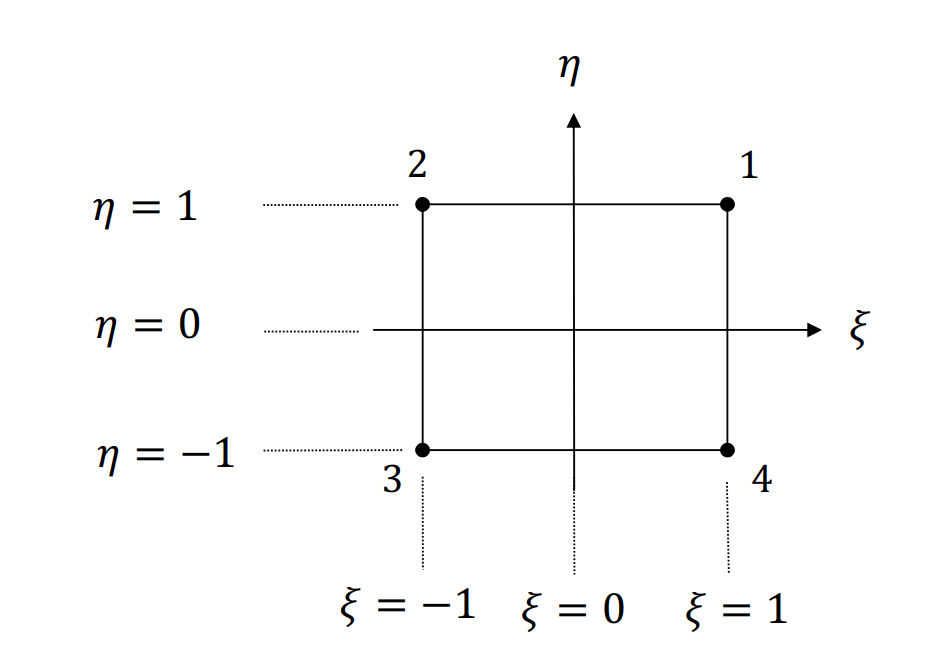
\includegraphics[width=0.6\textwidth,center]{fig/quadrilatero_4_livro.PNG}
	\caption{Parametrização de um elementos quadrilátero bilinear (4 nós)} 
	\label{cap6:quad_bilinear}
\end{figure}
%
as funções de interpolações bilineares são,
%
\begin{equation}
	\begin{split}
		&N_1(\xi, \eta) = \frac{1}{4}(1 + \xi)(1 + \eta)\\
		&N_2(\xi, \eta) = \frac{1}{4}(1 - \xi)(1 + \eta)\\
		&N_3(\xi, \eta) = \frac{1}{4}(1 - \xi)(1 - \eta)\\
		&N_4(\xi, \eta) = \frac{1}{4}(1 + \xi)(1 - \eta)
	\end{split}
\end{equation}
%
A as derivadas em relação a $\xi$ são,
\begin{equation}
	\begin{split}
		&\mdp{N_1}{\xi} = \frac{1}{4}(1 + \eta)\\
		&\mdp{N_2}{\xi} =-\frac{1}{4}(1 + \eta)\\
		&\mdp{N_3}{\xi} =-\frac{1}{4}(1 - \eta)\\
		&\mdp{N_4}{\xi} = \frac{1}{4}(1 - \eta)\\
	\end{split}
\end{equation}
%
e as derivadas em relação a $\eta$ são,
\begin{equation}
	\begin{split}
		&\mdp{N_1}{\eta} = \frac{1}{4}(1 + \xi)\\
		&\mdp{N_2}{\eta} = \frac{1}{4}(1 - \xi)\\
		&\mdp{N_3}{\eta} =-\frac{1}{4}(1 - \xi)\\
		&\mdp{N_4}{\eta} =-\frac{1}{4}(1 + \xi)\\
	\end{split}
\end{equation}
%
A deriva de $x$ em relação a  $\xi$ são,
%
\begin{equation}
	\begin{split}
&	\mdp{x}{\xi} = x_1 \mdp{N_1}{\xi} + x_2 \mdp{N_2}{\xi} + x_3 \mdp{N_3}{\xi} + x_4 \mdp{N_4}{\xi}\\
&   \mdp{x}{\xi} = \frac{x_1}{4} (1 + \eta) - \frac{x_2}{4} (1 + \eta) - \frac{x_1}{4} (1 - \eta) + \frac{x_4}{4} (1 - \eta)\\
&   \mdp{x}{\xi} = \frac{1}{4}\left[ (x_1 - x_2)(1 + \eta) + (x_4 - x_3)(1 - \eta) \right]
	\end{split}
\end{equation}
%
A deriva de $y$ em relação a  $\xi$ são,
%
\begin{equation}
	\begin{split}
		&	\mdp{y}{\xi} = y_1 \mdp{N_1}{\xi} + y_2 \mdp{N_2}{\xi} + y_3 \mdp{N_3}{\xi} + y_4 \mdp{N_4}{\xi}\\
		&   \mdp{y}{\xi} = \frac{1}{4}\left[ (y_1 - y_2)(1 + \eta) + (y_4 - y_3)(1 - \eta) \right]
	\end{split}
\end{equation}
%
A deriva de $x$ em relação a  $\eta$ são,
%
\begin{equation}
	\begin{split}
		&	\mdp{x}{\eta} = x_1 \mdp{N_1}{\eta} + x_2 \mdp{N_2}{\eta} + x_3 \mdp{N_3}{\eta} + x_4 \mdp{N_4}{\eta}\\
		&   \mdp{x}{\eta} = \frac{1}{4}\left[ (x_1 - x_4)(1 + \xi) + (x_2 - x_3)(1 - \xi) \right]
	\end{split}
\end{equation}
%
A deriva de $y$ em relação a  $\eta$ são,
%
\begin{equation}
	\begin{split}
		&	\mdp{y}{\eta} = y_1 \mdp{N_1}{\eta} + y_2 \mdp{N_2}{\eta} + y_3 \mdp{N_3}{\eta} + y_4 \mdp{N_4}{\eta}\\
		&   \mdp{y}{\eta} = \frac{1}{4}\left[ (y_1 - y_4)(1 + \xi) + (y_2 - y_3)(1 - \xi) \right]
	\end{split}
\end{equation}
%
Assim o operador jacobiano fica definido como,
%
\begin{equation}
	\begin{split}
&	\mdp{x}{\xi } = \frac{1}{4}\left[ (x_1 - x_2)(1 + \eta) + (x_4 - x_3)(1 - \eta) \right]\\
&   \mdp{y}{\xi } = \frac{1}{4}\left[ (y_1 - y_2)(1 + \eta) + (y_4 - y_3)(1 - \eta) \right]\\
&   \mdp{x}{\eta} = \frac{1}{4}\left[ (x_1 - x_4)(1 + \xi ) + (x_2 - x_3)(1 - \xi ) \right]\\
&   \mdp{y}{\eta} = \frac{1}{4}\left[ (y_1 - y_4)(1 + \xi ) + (y_2 - y_3)(1 - \xi ) \right]
	\end{split}
\end{equation}
%
Resolvendo agora as questões:
%
\begin{itemize}
	\item a)
	Considerando o ponto $P_3$ como referencia, temos as seguintes coordenadas para os pontos,
	%
	\begin{equation}
		\begin{split}
			&	P_1 = (x_3 + 6, y_3 + 4)\\
			&	P_2 = (x_3    , y_3 + 4)\\
			&	P_3 = (x_3    , y_3    )\\
			&	P_4 = (x_3 + 6, y_3    )\\
		\end{split}
	\end{equation}
	%
	Nos temos agora que para os $xs$,
	\begin{equation}
		\begin{split}
			&	(x_1 - x_2) = x_3 + 6 - x_3 = 6 \\
			&	(x_4 - x_3) = x_3 + 6 - x_3 = 6\\
			&	(x_1 - x_4) = x_3 + 6 - (x_3 + 6) = 0\\\
			&	(x_2 - x_3) = x_3 - x_3 = 0\\
		\end{split}
	\end{equation}
	%
	e para os $ys$,
	\begin{equation}
	\begin{split}
		&	(y_1 - y_2) = y_3 + 4 - (y_3 + 4) = 0 \\
		&	(y_4 - y_3) = y_3 - y_3 = 0\\
		&	(y_1 - y_4) = y_3 + 4 - y_3 = 4\\\
		&	(y_2 - y_3) = y_3 + 4 - y_3 = 4\\
	\end{split}
	\end{equation}
	%
	\begin{equation}
		\begin{split}
			&	\mdp{x}{\xi } = \frac{1}{4}\left[ 6(1 + \eta) + 6(1 - \eta) \right] = 3\\
			&   \mdp{y}{\xi } = \frac{1}{4}\left[ 0(1 + \eta) + 0(1 - \eta) \right] = 0\\
			&   \mdp{x}{\eta} = \frac{1}{4}\left[ 0(1 + \xi ) + 0(1 - \xi ) \right] = 0\\
			&   \mdp{y}{\eta} = \frac{1}{4}\left[ 4(1 + \xi ) + 4(1 - \xi ) \right] = 2
		\end{split}
	\end{equation}
	%
	Portando o operador Jacobiano é dado por,

	\color{blue}
	\textbf{Resposta:}
	\begin{equation}
	J(\xi, \eta) = 
	\begin{bmatrix}
		3 & 0\\
		0 & 2\\
	\end{bmatrix}
	\end{equation}	
	\color{black}
	% 
	Pode-se checar o resultado através do calculo da área do elemento,
	\begin{equation}
		\begin{split}
		& A = b * h = \int_A dA = \int_{-1}^1 \int_{-1}^1 det J d\xi d\eta\\
		& 4 * 6 = \int_{-1}^1 \int_{-1}^1 \left(3 * 2\right)  d\xi d\eta\\
		& 4 * 6 = 6 * 2 * 2 \\
		& 24 = 24		
		\end{split}
	\end{equation}
	%	
	\item b)
	Considerando o ponto $P_3$ como referencia, temos as seguintes coordenadas para os pontos,
	%
	\begin{equation}
		\begin{split}
		&	P_1 = (x_3 + 7, y_3 + 2)\\
		&	P_2 = (x_3 + 1, y_3 + 2)\\
		&	P_3 = (x_3    , y_3    )\\
		&	P_4 = (x_3 + 6, y_3    )\\
		\end{split}
	\end{equation}
	%
	Nos temos agora que para os $xs$,
	\begin{equation}
	\begin{split}
		&	(x_1 - x_2) = x_3 + 7 - (x_3 + 1) = 6 \\
		&	(x_4 - x_3) = x_3 + 6 - x_3 = 6\\
		&	(x_1 - x_4) = x_3 + 7 - (x_3 + 6) = 1\\\
		&	(x_2 - x_3) = x_3 + 1 - x_3 = 1\\
	\end{split}
	\end{equation}
	%
	e para os $ys$,
	\begin{equation}
	\begin{split}
		&	(y_1 - y_2) = y_3 + 2 - (y_3 + 2) = 0 \\
		&	(y_4 - y_3) = y_3 - y_3 = 0\\
		&	(y_1 - y_4) = y_3 + 2 - y_3 = 2\\\
		&	(y_2 - y_3) = y_3 + 2 - y_3 = 2\\
	\end{split}
	\end{equation}
	%
	\begin{equation}
	\begin{split}
		&	\mdp{x}{\xi } = \frac{1}{4}\left[ 6(1 + \eta) + 6(1 - \eta) \right] = 3\\
		&   \mdp{y}{\xi } = \frac{1}{4}\left[ 0(1 + \eta) + 0(1 - \eta) \right] = 0\\
		&   \mdp{x}{\eta} = \frac{1}{4}\left[ 1(1 + \xi ) + 1(1 - \xi ) \right] = \frac{1}{2}\\
		&   \mdp{y}{\eta} = \frac{1}{4}\left[ 2(1 + \xi ) + 2(1 - \xi ) \right] = 1
	\end{split}
	\end{equation}
	%
	Portando o operador Jacobiano é dado por,

	\color{blue}
	\textbf{Resposta:}
	\begin{equation}
	J(\xi, \eta) = 
	\begin{bmatrix}
		3 & 0\\
		\frac{1}{2} & 1\\
	\end{bmatrix}
	\end{equation}	
	\color{black}
	% 
	Pode-se checar o resultado através do calculo da área do elemento,
	\begin{equation}
		\begin{split}
		& A = b * h = \int_A dA = \int_{-1}^1 \int_{-1}^1 det J d\xi d\eta\\
		& 2 * 6 = \int_{-1}^1 \int_{-1}^1 \left(3 * 1\right)  d\xi d\eta\\
		& 2 * 6 = 3 * 2 * 2 \\
		& 12 = 12		
		\end{split}
	\end{equation}
	%
	%	
	\item c)
	Considerando o ponto $P_3$ como referencia, temos as seguintes coordenadas para os pontos,
	%
	\begin{equation}
		\begin{split}
			&	P_1 = (x_3 + 2, y_3 + 2)\\
			&	P_2 = (x_3    , y_3 + 1)\\
			&	P_3 = (x_3    , y_3    )\\
			&	P_4 = (x_3 + 2, y_3    )\\
		\end{split}
	\end{equation}
	%
	Nos temos agora que para os $xs$,
	\begin{equation}
		\begin{split}
			&	(x_1 - x_2) = x_3 + 2 - x_3 = 2 \\
			&	(x_4 - x_3) = x_3 + 2 - x_3 = 2\\
			&	(x_1 - x_4) = x_3 + 2 - (x_3 + 2) = 0\\\
			&	(x_2 - x_3) = x_3  - x_3 = 0\\
		\end{split}
	\end{equation}
	%
	e para os $ys$,
	\begin{equation}
		\begin{split}
			&	(y_1 - y_2) = y_3 + 2 - (y_3 + 1) = 1 \\
			&	(y_4 - y_3) = y_3 - y_3 = 0\\
			&	(y_1 - y_4) = y_3 + 2 - y_3 = 2\\\
			&	(y_2 - y_3) = y_3 + 1 - y_3 = 1\\
		\end{split}
	\end{equation}
	%
	\begin{equation}
		\begin{split}
			&	\mdp{x}{\xi } = \frac{1}{4}\left[ 2(1 + \eta) + 2(1 - \eta) \right] = 1\\
			&   \mdp{y}{\xi } = \frac{1}{4}\left[ 1(1 + \eta) + 2(1 - \eta) \right] = \frac{3 - \eta}{4}\\
			&   \mdp{x}{\eta} = \frac{1}{4}\left[ 0(1 + \xi ) + 0(1 - \xi ) \right] = 0\\
			&   \mdp{y}{\eta} = \frac{1}{4}\left[ 2(1 + \xi ) + 1(1 - \xi ) \right] = \frac{3 + \xi}{4}
		\end{split}
	\end{equation}
	%
	Portando o operador Jacobiano é dado por,
	
	\color{blue}
	\textbf{Resposta:}
	\begin{equation}
		J(\xi, \eta) = 
		\begin{bmatrix}
			1 & \frac{3 - \eta}{4}\\
			0 & \frac{3 + \xi}{4}\\
		\end{bmatrix}
	\end{equation}	
	\color{black}
	% 
	Pode-se checar o resultado através do calculo da área do elemento,
	\begin{equation}
		\begin{split}
			& A = \frac{(b + B) * h}{2} = \int_A dA = \int_{-1}^1 \int_{-1}^1 det J d\xi d\eta\\
			& \frac{(1 + 2) * 2}{2} = \int_{-1}^1 \int_{-1}^1 \left(\frac{3 + \xi}{4}\right)  d\xi d\eta\\
			& \frac{3 * 2}{2} = \frac{1}{4} * 2 * 6 \\
			& 3 = 3		
		\end{split}
	\end{equation}		
%
\end{itemize}
%
\subsubsection{4) Determine as funções de interpolação de um hexaedro quadrático}
%
\begin{figure}[H]
		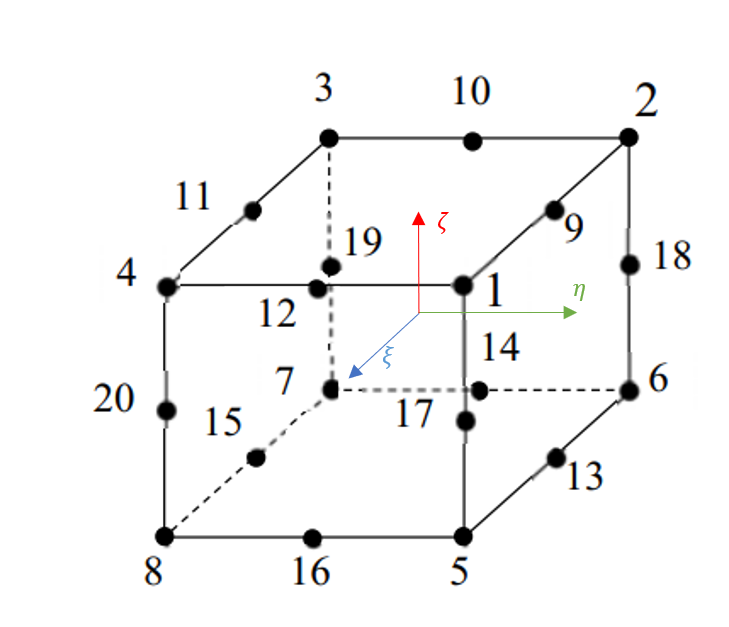
\includegraphics[width=0.6\textwidth,center]{fig/hexaedro_20.PNG}
		\caption{Hexaedros 20 nós} 
\end{figure}
%
Pontos $(\xi,\eta,\zeta)$,
%
\begin{equation*}
		\begin{matrix}
		P_1 = ( 1, 1, 1)	& P_5 = ( 1, 1,-1)&P_{17} = ( 1, 1,0)\\ 
		P_2 = (-1, 1, 1)	& P_6 = (-1, 1,-1)&P_{18} = (-1, 1,0)\\
		P_3 = (-1,-1, 1)    & P_7 = (-1,-1,-1)&P_{19} = (-1,-1,0)\\ 
		P_4 = ( 1,-1, 1)    & P_8 = ( 1,-1,-1)&P_{20} = ( 1,-1,0)
		\end{matrix}
\end{equation*}
%
\begin{equation*}
	\begin{matrix}
	P_9    = (  0, 1, 1) &P_{13} = ( 0, 1, -1)\\
	P_{10} = ( -1, 0, 1) &P_{14} = (-1, 0, -1)\\
	P_{11} = (  0,-1, 1) &P_{15} = ( 0,-1, -1)\\
	P_{12} = (  1, 0, 1) &P_{16} = ( 1, 0, -1)
	\end{matrix}
\end{equation*}
%
Funções de interpolações:
%
\begin{equation}
	\begin{split}
		& N_1 = \frac{1}{8}(1+\xi)(1+\eta)(1+\zeta)( \xi + \eta + \zeta - 2)\\
		& N_2 = \frac{1}{8}(1-\xi)(1+\eta)(1+\zeta)(-\xi + \eta + \zeta - 2)\\
		& N_3 = \frac{1}{8}(1-\xi)(1-\eta)(1+\zeta)(-\xi - \eta + \zeta - 2)\\
		& N_4 = \frac{1}{8}(1+\xi)(1-\eta)(1+\zeta)(-\xi + \eta + \zeta - 2)\\	
		& N_5 = \frac{1}{8}(1+\xi)(1+\eta)(1-\zeta)( \xi + \eta - \zeta - 2)\\
		& N_6 = \frac{1}{8}(1-\xi)(1+\eta)(1-\zeta)(-\xi + \eta - \zeta - 2)\\
		& N_7 = \frac{1}{8}(1-\xi)(1-\eta)(1-\zeta)(-\xi - \eta - \zeta - 2)\\
		& N_8 = \frac{1}{8}(1+\xi)(1-\eta)(1-\zeta)(-\xi + \eta - \zeta - 2)\\	
		& N_9    = \frac{1}{4}(1-\xi^2)(1+\eta)(1+\zeta)\\
		& N_{11} = \frac{1}{4}(1-\xi^2)(1-\eta)(1+\zeta)\\
		& N_{13} = \frac{1}{4}(1-\xi^2)(1+\eta)(1-\zeta)\\
		& N_{15} = \frac{1}{4}(1-\xi^2)(1-\eta)(1-\zeta)\\
		& N_{10} = \frac{1}{4}(1-\eta^2)(1-\xi)(1+\zeta)\\
		& N_{12} = \frac{1}{4}(1-\eta^2)(1+\xi)(1+\zeta)\\
		& N_{14} = \frac{1}{4}(1-\eta^2)(1-\xi)(1-\zeta)\\	
		& N_{16} = \frac{1}{4}(1-\eta^2)(1+\xi)(1-\zeta)\\		
		& N_{17} = \frac{1}{4}(1-\zeta^2)(1+\xi)(1+\eta)\\
		& N_{18} = \frac{1}{4}(1-\zeta^2)(1-\xi)(1+\eta)\\
		& N_{19} = \frac{1}{4}(1-\zeta^2)(1-\xi)(1-\eta)\\	
		& N_{20} = \frac{1}{4}(1-\zeta^2)(1+\xi)(1-\eta)\\	
	\end{split}
\end{equation}	
%
\subsubsection{5) Calcular as forças nodais equivalentes para os elementos de elasticidades plana abaixo, considerando uma distribuição uniforme de forças de volume na direção y}

A integral de forças de volume é(pag. 22),
%
\begin{equation}
\mathbf{f}_i = \int_{\Omega} \mathbf{N}_i \mathbf{b} d\Omega
\end{equation}
%
em notação matricial temos,
%
\begin{equation}
	\begin{bmatrix}
	f^x_i\\
	f^y_i\\
	\end{bmatrix}
	=
	\int_{\Omega}
	\begin{bmatrix}
	N_i&0\\
	0&N_i\\
	\end{bmatrix}
	\begin{bmatrix}
	b_x\\
	b_y\\
	\end{bmatrix}
	d\Omega
	=
	\int_{\Omega}
	\begin{bmatrix}
		N_i b_x\\
		N_i b_y\\
	\end{bmatrix}
	d\Omega
	=
	\begin{bmatrix}
	\int_{\Omega} N_i b_x d\Omega\\
	\int_{\Omega} N_i b_y d\Omega\\
	\end{bmatrix}
\end{equation}
%
Como $b_x$ é igual 0, temos,
%
\begin{equation}
	\begin{bmatrix}
		f^x_i\\
		f^y_i\\
	\end{bmatrix}
	=
	\begin{bmatrix}
		0\\
		\int_{\Omega} N_i b_y d\Omega\\
	\end{bmatrix}
\end{equation}
%
É necessário calcular a integral em relação a $N_i$, lembrando que a integral é em relação ao sistema de coordenadas x-y,
%
\begin{equation}
\int_{\Omega} N_i(x,y) d\Omega
\end{equation}
%
A integral usando as coordenadas locais no elemento triangular é,
%
\begin{equation}
	\int_{\Omega} N_i(x,y) d\Omega = \int_{0}^{1} \int_{0}^{1-\xi_1}  N_i(\xi_1,\xi_2) det J d \xi_1 d \xi_2 
\end{equation}
%
Considerando uma interpolação linear para geometria o determinante do jacobiano é constante e igual a duas vezes a área do triangulo, portando,
%
\begin{equation}
	\int_{\Omega} N_i(x,y) d\Omega = 2 A \int_{0}^{1} \int_{0}^{1-\xi_1}  N_i(\xi_1,\xi_2) d \xi_1 d \xi_2 = 2 A f_i
\end{equation}
%
Para resolver o problema precisamos apenas calcular essas integrais.

\begin{itemize}
	\item a)
	Para o triangulo linear temos as seguintes funções de interpolação
	%
	\begin{equation}
		\begin{split}
		&N_1 = \xi_1\\ 
		&N_2 = \xi_2\\ 
		&N_3 = 1 - \xi_1 - \xi_2\\ 
		\end{split}
	\end{equation}
	%	
	A integrais ficam
	%
	\begin{equation}
		\begin{split}
			&f_1 = \int_{0}^{1} \int_{0}^{1-\xi_1}  N_1 d \xi_1 d \xi_2 = \int_{0}^{1} \int_{0}^{1-\xi_1}  \xi_1 d \xi_1 d \xi_2 = \frac{1}{6}\\ 
			&f_2 = \int_{0}^{1} \int_{0}^{1-\xi_1}  N_2 d \xi_1 d \xi_2 = \int_{0}^{1} \int_{0}^{1-\xi_1}  \xi_2 d \xi_1 d \xi_2 = \frac{1}{6}\\ 
			&f_3 = \int_{0}^{1} \int_{0}^{1-\xi_1}  N_3 d \xi_1 d \xi_2 = \int_{0}^{1} \int_{0}^{1-\xi_1}  1 - \xi_1 - \xi_2 d \xi_1 d \xi_2 = \frac{1}{6} 
		\end{split}
	\end{equation}
	%
	Portanto
	\begin{equation}
		\begin{split}
			&f_1^y = (b_y) (2 A) \left(\frac{1}{6}\right) = \frac{b_y A}{3}\\ 
			&f_2^y = (b_y) (2 A) \left(\frac{1}{6}\right) = \frac{b_y A}{3}\\ 
			&f_3^y = (b_y) (2 A) \left(\frac{1}{6}\right) = \frac{b_y A}{3} 
		\end{split}
	\end{equation}
	% 
	Assim os vetores de força equivalentes é dados por,

	\color{blue}
	\textbf{Resposta:}
	\begin{equation}
		\mathbf{f}_1 = \mathbf{f}_2 = \mathbf{f}_3
		=
		\frac{b_y A}{3}
		\begin{bmatrix}
			0\\
			1
		\end{bmatrix}
	\end{equation}
	\color{black}
	%
	
	\item b)
	Para o triangulo quadrático temos as seguintes funções de interpolação
	%
	\begin{equation}
		\begin{split}
			&N_1 = \xi_1(2\xi_1 - 1)\\ 
			&N_2 = \xi_2(2\xi_2 - 1)\\ 
			&N_3 = \xi_3(2\xi_3 - 1)\\ 
			&N_4 = 4 \xi_1 \xi_2\\ 
			&N_5 = 4 \xi_2 \xi_3\\ 
			&N_6 = 4 \xi_3 \xi_1 
		\end{split}
	\end{equation}
	%	
	A integrais ficam
	%
	\begin{equation}
		\begin{split}
			&f_1 = \int_{0}^{1} \int_{0}^{1-\xi_1}  N_1 d \xi_1 d \xi_2 = 0\\ 
			&f_2 = \int_{0}^{1} \int_{0}^{1-\xi_1}  N_2 d \xi_1 d \xi_2 = 0\\ 
			&f_3 = \int_{0}^{1} \int_{0}^{1-\xi_1}  N_3 d \xi_1 d \xi_2 = 0\\ 
			&f_4 = \int_{0}^{1} \int_{0}^{1-\xi_1}  N_1 d \xi_1 d \xi_2 = \frac{1}{6}\\ 
			&f_5 = \int_{0}^{1} \int_{0}^{1-\xi_1}  N_2 d \xi_1 d \xi_2 = \frac{1}{6}\\ 
			&f_6 = \int_{0}^{1} \int_{0}^{1-\xi_1}  N_3 d \xi_1 d \xi_2 = \frac{1}{6} 
		\end{split}
	\end{equation}
	%	
	Portanto
	\begin{equation}
	\begin{split}
		&f_1^y = 0\\ 
		&f_2^y = 0\\ 
		&f_3^y = 0\\
		&f_4^y = \frac{b_y A}{3}\\ 
		&f_5^y = \frac{b_y A}{3}\\ 
		&f_6^y = \frac{b_y A}{3}  
	\end{split}
	\end{equation}
	% 
	Assim os vetores de força equivalentes é dados por,

	\color{blue}
	\textbf{Resposta:}
	\begin{equation}
	\begin{split}
		&\mathbf{f}_1 = \mathbf{f}_2 = \mathbf{f}_3 =
		\begin{bmatrix}
			0\\
			0
		\end{bmatrix}\\
		&\mathbf{f}_4 = \mathbf{f}_5 = \mathbf{f}_6  
		=
		\frac{b_y A}{3}
		\begin{bmatrix}
			0\\
			1
		\end{bmatrix}
		\end{split}
	\end{equation}
	\color{black}
%
%
\end{itemize}

\subsubsection{6) Calcular as forças nodais equivalentes para os elementos quadriláteros quadrático de elasticidade plana}

A integral de forças de volume é(pag. 22),
%
\begin{equation}
	\mathbf{f}_i = \int_{\Gamma} \mathbf{N}_i \mathbf{\bar t} d\Gamma
\end{equation}
%
em notação matricial temos,
%
\begin{equation}
	\begin{bmatrix}
		f^x_i\\
		f^y_i\\
	\end{bmatrix}
	=
	\int_{\Gamma}
	\begin{bmatrix}
		N_i&0\\
		0&N_i\\
	\end{bmatrix}
	\begin{bmatrix}
		q_x\\
		q_y\\
	\end{bmatrix}
	d\Gamma
	=
	\int_{\Gamma}
	\begin{bmatrix}
		N_i q_x\\
		N_i q_y\\
	\end{bmatrix}
	d\Gamma
	=
	\begin{bmatrix}
		\int_{\Gamma} N_i q_x d\Gamma\\
		\int_{\Gamma} N_i q_y d\Gamma
	\end{bmatrix}
\end{equation}
%
Como a força são uniformes nos bordos,
%
\begin{equation}
	\begin{bmatrix}
		f^x_i\\
		f^y_i\\
	\end{bmatrix}
	=
	\begin{bmatrix}
		q_x \int_{\Gamma} N_i d\Gamma\\
		q_y \int_{\Gamma} N_i d\Gamma
	\end{bmatrix}
\end{equation}
%
Portanto temos,
%
\begin{equation}
\begin{split}
&f^x_2 = q_x \int_{\Gamma} N_2 d\Gamma \quad f^y_2 = 0\\
&f^x_6 = q_x \int_{\Gamma} N_6 d\Gamma \quad f^y_6 = 0\\
&f^x_3 = q_x \int_{\Gamma} N_3 d\Gamma \quad f^y_3 =  q_y \int_{\Gamma} N_3 d\Gamma\\
&f^x_7 = 0 \quad f^y_7 =  q_y \int_{\Gamma} N_7 d\Gamma\\
&f^x_4 = 0 \quad f^y_4 = q_y \int_{\Gamma} N_4 d\Gamma
\end{split}
\end{equation}
%
Como a integral é apenas nos bordos, na aresta 2-3 temos, as seguintes funções de interpolações 
%
\begin{equation}
	\begin{split}
		&N_2 = \frac{1}{2} \eta (1 + \eta) \\ 
		&N_6 = (1 + \eta) (1 - \eta) \\ 
		&N_3 = \frac{1}{2} \eta (\eta - 1)  
	\end{split}
\end{equation}
%
As integrais são,
\begin{equation}
	\begin{split}
		&\int_{\Gamma} N_2 d\Gamma = \int_{-1}^{1} N_2 det J d\eta = \frac{L}{2} \int_{-1}^{1} N_2 d\eta =  \frac{L}{6}\\
		&\int_{\Gamma} N_6 d\Gamma = \int_{-1}^{1} N_6 det J d\eta = \frac{L}{2} \int_{-1}^{1} N_6 d\eta =  \frac{2 L}{3}\\
		&\int_{\Gamma} N_3 d\Gamma = \int_{-1}^{1} N_3 det J d\eta = \frac{L}{2} \int_{-1}^{1} N_3 d\eta =  \frac{L}{6}
	\end{split}
\end{equation}
Como a integral é apenas nos bordos, na aresta 3-4 temos, as seguintes funções de interpolações 
%
\begin{equation}
	\begin{split}
		&N_3 = \frac{1}{2} \xi (\xi - 1) \\ 
		&N_7 = (1 + \xi) (1 - \xi) \\ 
		&N_4 = \frac{1}{2} \xi (1 + \xi)  
	\end{split}
\end{equation}
%
As integrais são,
\begin{equation}
	\begin{split}
		&\int_{\Gamma} N_3 d\Gamma = \int_{-1}^{1} N_3 det J d\eta = \frac{L}{2} \int_{-1}^{1} N_3 d\eta =  \frac{L}{6}\\
		&\int_{\Gamma} N_7 d\Gamma = \int_{-1}^{1} N_7 det J d\eta = \frac{L}{2} \int_{-1}^{1} N_7 d\eta =  \frac{2 L}{3}\\
		&\int_{\Gamma} N_4 d\Gamma = \int_{-1}^{1} N_4 det J d\eta = \frac{L}{2} \int_{-1}^{1} N_4 d\eta =  \frac{L}{6}
	\end{split}
\end{equation}
%
Portanto temos,
%
\begin{equation}
	\begin{split}
		&f^x_2 = \frac{q_x L}{6} \quad f^y_2 = 0\\
		&f^x_6 = \frac{2 q_x L}{3} \quad f^y_6 = 0\\
		&f^x_3 = \frac{q_x L}{6} \quad f^y_3 = \frac{q_y L}{6}\\
		&f^x_7 = 0 \quad f^y_7 = \frac{2 q_y L}{3}\\
		&f^x_4 = 0 \quad f^y_4 = \frac{q_y L}{6}
	\end{split}
\end{equation}
%
\color{blue}
\textbf{Resposta:}
\begin{equation}
	\begin{split}
		&\mathbf{f}_2 =
		\begin{bmatrix}
			\frac{q_x L}{6}\\
			0
		\end{bmatrix}\\
		&\mathbf{f}_3 =
		\begin{bmatrix}
		\frac{q_x L}{6}\\
		\frac{q_y L}{6}
		\end{bmatrix}\\
		&\mathbf{f}_4 =
		\begin{bmatrix}
		0\\
		\frac{q_y L}{6}
		\end{bmatrix}\\
		&\mathbf{f}_6 =
		\begin{bmatrix}
		\frac{2 q_x L}{3}\\
		0
		\end{bmatrix}\\
		&\mathbf{f}_7 =
		\begin{bmatrix}
		0\\
		\frac{2 q_y L}{3}
		\end{bmatrix}
	\end{split}
\end{equation}
\color{black}


